\documentclass[1p]{elsarticle_modified}
%\bibliographystyle{elsarticle-num}

%\usepackage[colorlinks]{hyperref}
%\usepackage{abbrmath_seonhwa} %\Abb, \Ascr, \Acal ,\Abf, \Afrak
\usepackage{amsfonts}
\usepackage{amssymb}
\usepackage{amsmath}
\usepackage{amsthm}
\usepackage{scalefnt}
\usepackage{amsbsy}
\usepackage{kotex}
\usepackage{caption}
\usepackage{subfig}
\usepackage{color}
\usepackage{graphicx}
\usepackage{xcolor} %% white, black, red, green, blue, cyan, magenta, yellow
\usepackage{float}
\usepackage{setspace}
\usepackage{hyperref}

\usepackage{tikz}
\usetikzlibrary{arrows}

\usepackage{multirow}
\usepackage{array} % fixed length table
\usepackage{hhline}

%%%%%%%%%%%%%%%%%%%%%
\makeatletter
\renewcommand*\env@matrix[1][\arraystretch]{%
	\edef\arraystretch{#1}%
	\hskip -\arraycolsep
	\let\@ifnextchar\new@ifnextchar
	\array{*\c@MaxMatrixCols c}}
\makeatother %https://tex.stackexchange.com/questions/14071/how-can-i-increase-the-line-spacing-in-a-matrix
%%%%%%%%%%%%%%%

\usepackage[normalem]{ulem}

\newcommand{\msout}[1]{\ifmmode\text{\sout{\ensuremath{#1}}}\else\sout{#1}\fi}
%SOURCE: \msout is \stkout macro in https://tex.stackexchange.com/questions/20609/strikeout-in-math-mode

\newcommand{\cancel}[1]{
	\ifmmode
	{\color{red}\msout{#1}}
	\else
	{\color{red}\sout{#1}}
	\fi
}

\newcommand{\add}[1]{
	{\color{blue}\uwave{#1}}
}

\newcommand{\replace}[2]{
	\ifmmode
	{\color{red}\msout{#1}}{\color{blue}\uwave{#2}}
	\else
	{\color{red}\sout{#1}}{\color{blue}\uwave{#2}}
	\fi
}

\newcommand{\Sol}{\mathcal{S}} %segment
\newcommand{\D}{D} %diagram
\newcommand{\A}{\mathcal{A}} %arc


%%%%%%%%%%%%%%%%%%%%%%%%%%%%%5 test

\def\sl{\operatorname{\textup{SL}}(2,\Cbb)}
\def\psl{\operatorname{\textup{PSL}}(2,\Cbb)}
\def\quan{\mkern 1mu \triangleright \mkern 1mu}

\theoremstyle{definition}
\newtheorem{thm}{Theorem}[section]
\newtheorem{prop}[thm]{Proposition}
\newtheorem{lem}[thm]{Lemma}
\newtheorem{ques}[thm]{Question}
\newtheorem{cor}[thm]{Corollary}
\newtheorem{defn}[thm]{Definition}
\newtheorem{exam}[thm]{Example}
\newtheorem{rmk}[thm]{Remark}
\newtheorem{alg}[thm]{Algorithm}

\newcommand{\I}{\sqrt{-1}}
\begin{document}

%\begin{frontmatter}
%
%\title{Boundary parabolic representations of knots up to 8 crossings}
%
%%% Group authors per affiliation:
%\author{Yunhi Cho} 
%\address{Department of Mathematics, University of Seoul, Seoul, Korea}
%\ead{yhcho@uos.ac.kr}
%
%
%\author{Seonhwa Kim} %\fnref{s_kim}}
%\address{Center for Geometry and Physics, Institute for Basic Science, Pohang, 37673, Korea}
%\ead{ryeona17@ibs.re.kr}
%
%\author{Hyuk Kim}
%\address{Department of Mathematical Sciences, Seoul National University, Seoul 08826, Korea}
%\ead{hyukkim@snu.ac.kr}
%
%\author{Seokbeom Yoon}
%\address{Department of Mathematical Sciences, Seoul National University, Seoul, 08826,  Korea}
%\ead{sbyoon15@snu.ac.kr}
%
%\begin{abstract}
%We find all boundary parabolic representation of knots up to 8 crossings.
%
%\end{abstract}
%\begin{keyword}
%    \MSC[2010] 57M25 
%\end{keyword}
%
%\end{frontmatter}

%\linenumbers
%\tableofcontents
%
\newcommand\colored[1]{\textcolor{white}{\rule[-0.35ex]{0.8em}{1.4ex}}\kern-0.8em\color{red} #1}%
%\newcommand\colored[1]{\textcolor{white}{ #1}\kern-2.17ex	\textcolor{white}{ #1}\kern-1.81ex	\textcolor{white}{ #1}\kern-2.15ex\color{red}#1	}

{\Large $\underline{12a_{0728}~(K12a_{0728})}$}

\setlength{\tabcolsep}{10pt}
\renewcommand{\arraystretch}{1.6}
\vspace{1cm}\begin{tabular}{m{100pt}>{\centering\arraybackslash}m{274pt}}
\multirow{5}{120pt}{
	\centering
	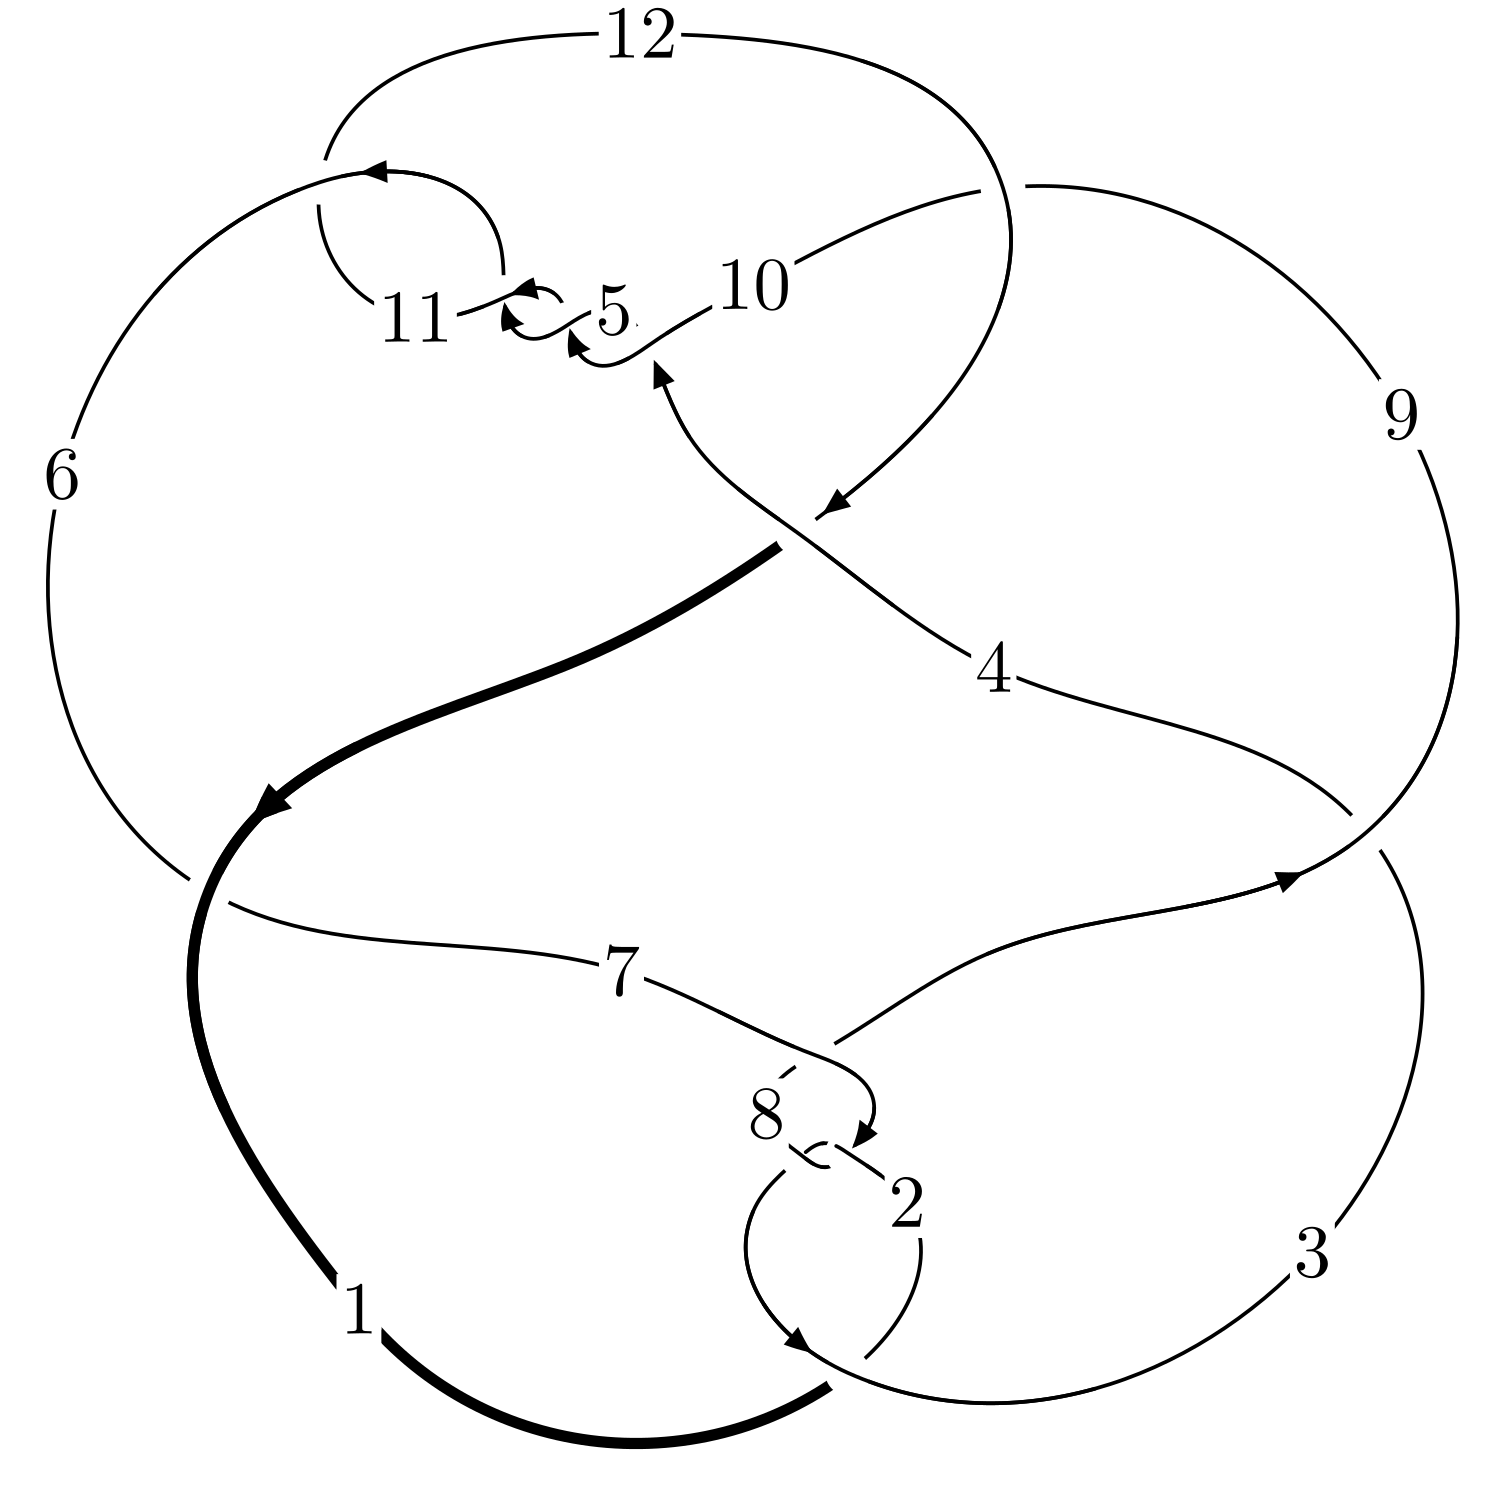
\includegraphics[width=112pt]{../../../GIT/diagram.site/Diagrams/png/1529_12a_0728.png}\\
\ \ \ A knot diagram\footnotemark}&
\allowdisplaybreaks
\textbf{Linearized knot diagam} \\
\cline{2-2}
 &
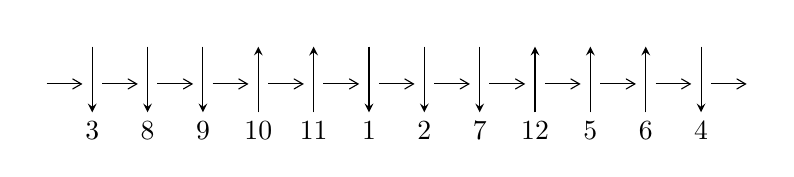
\begin{tikzpicture}[x=20pt, y=17pt]
	% nodes
	\node (C0) at (0, 0) {};
	\node (C1) at (1, 0) {};
	\node (C1U) at (1, +1) {};
	\node (C1D) at (1, -1) {3};

	\node (C2) at (2, 0) {};
	\node (C2U) at (2, +1) {};
	\node (C2D) at (2, -1) {8};

	\node (C3) at (3, 0) {};
	\node (C3U) at (3, +1) {};
	\node (C3D) at (3, -1) {9};

	\node (C4) at (4, 0) {};
	\node (C4U) at (4, +1) {};
	\node (C4D) at (4, -1) {10};

	\node (C5) at (5, 0) {};
	\node (C5U) at (5, +1) {};
	\node (C5D) at (5, -1) {11};

	\node (C6) at (6, 0) {};
	\node (C6U) at (6, +1) {};
	\node (C6D) at (6, -1) {1};

	\node (C7) at (7, 0) {};
	\node (C7U) at (7, +1) {};
	\node (C7D) at (7, -1) {2};

	\node (C8) at (8, 0) {};
	\node (C8U) at (8, +1) {};
	\node (C8D) at (8, -1) {7};

	\node (C9) at (9, 0) {};
	\node (C9U) at (9, +1) {};
	\node (C9D) at (9, -1) {12};

	\node (C10) at (10, 0) {};
	\node (C10U) at (10, +1) {};
	\node (C10D) at (10, -1) {5};

	\node (C11) at (11, 0) {};
	\node (C11U) at (11, +1) {};
	\node (C11D) at (11, -1) {6};

	\node (C12) at (12, 0) {};
	\node (C12U) at (12, +1) {};
	\node (C12D) at (12, -1) {4};
	\node (C13) at (13, 0) {};

	% arrows
	\draw[->,>={angle 60}]
	(C0) edge (C1) (C1) edge (C2) (C2) edge (C3) (C3) edge (C4) (C4) edge (C5) (C5) edge (C6) (C6) edge (C7) (C7) edge (C8) (C8) edge (C9) (C9) edge (C10) (C10) edge (C11) (C11) edge (C12) (C12) edge (C13) ;	\draw[->,>=stealth]
	(C1U) edge (C1D) (C2U) edge (C2D) (C3U) edge (C3D) (C4D) edge (C4U) (C5D) edge (C5U) (C6U) edge (C6D) (C7U) edge (C7D) (C8U) edge (C8D) (C9D) edge (C9U) (C10D) edge (C10U) (C11D) edge (C11U) (C12U) edge (C12D) ;
	\end{tikzpicture} \\
\hhline{~~} \\& 
\textbf{Solving Sequence} \\ \cline{2-2} 
 &
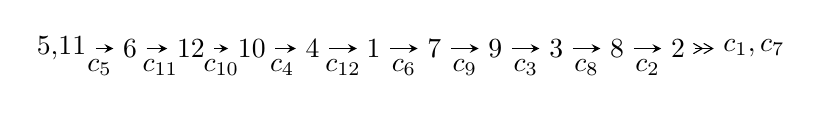
\begin{tikzpicture}[x=22pt, y=7pt]
	% node
	\node (A0) at (-1/8, 0) {5,11};
	\node (A1) at (1, 0) {6};
	\node (A2) at (2, 0) {12};
	\node (A3) at (3, 0) {10};
	\node (A4) at (4, 0) {4};
	\node (A5) at (5, 0) {1};
	\node (A6) at (6, 0) {7};
	\node (A7) at (7, 0) {9};
	\node (A8) at (8, 0) {3};
	\node (A9) at (9, 0) {8};
	\node (A10) at (10, 0) {2};
	\node (C1) at (1/2, -1) {$c_{5}$};
	\node (C2) at (3/2, -1) {$c_{11}$};
	\node (C3) at (5/2, -1) {$c_{10}$};
	\node (C4) at (7/2, -1) {$c_{4}$};
	\node (C5) at (9/2, -1) {$c_{12}$};
	\node (C6) at (11/2, -1) {$c_{6}$};
	\node (C7) at (13/2, -1) {$c_{9}$};
	\node (C8) at (15/2, -1) {$c_{3}$};
	\node (C9) at (17/2, -1) {$c_{8}$};
	\node (C10) at (19/2, -1) {$c_{2}$};
	\node (A11) at (45/4, 0) {$c_{1},c_{7}$};

	% edge
	\draw[->,>=stealth]	
	(A0) edge (A1) (A1) edge (A2) (A2) edge (A3) (A3) edge (A4) (A4) edge (A5) (A5) edge (A6) (A6) edge (A7) (A7) edge (A8) (A8) edge (A9) (A9) edge (A10) ;
	\draw[->>,>={angle 60}]	
	(A10) edge (A11);
\end{tikzpicture} \\ 

\end{tabular} \\

\footnotetext{
The image of knot diagram is generated by the software ``\textbf{Draw programme}" developed by Andrew Bartholomew(\url{http://www.layer8.co.uk/maths/draw/index.htm\#Running-draw}), where we modified some parts for our purpose(\url{https://github.com/CATsTAILs/LinksPainter}).
}\phantom \\ \newline 
\centering \textbf{Ideals for irreducible components\footnotemark of $X_{\text{par}}$} 
 
\begin{align*}
I^u_{1}&=\langle 
u^{66}+u^{65}+\cdots+u+1\rangle \\
\\
\end{align*}
\raggedright * 1 irreducible components of $\dim_{\mathbb{C}}=0$, with total 66 representations.\\
\footnotetext{All coefficients of polynomials are rational numbers. But the coefficients are sometimes approximated in decimal forms when there is not enough margin.}
\newpage
\renewcommand{\arraystretch}{1}
\centering \section*{I. $I^u_{1}= \langle u^{66}+u^{65}+\cdots+u+1 \rangle$}
\flushleft \textbf{(i) Arc colorings}\\
\begin{tabular}{m{7pt} m{180pt} m{7pt} m{180pt} }
\flushright $a_{5}=$&$\begin{pmatrix}1\\0\end{pmatrix}$ \\
\flushright $a_{11}=$&$\begin{pmatrix}0\\u\end{pmatrix}$ \\
\flushright $a_{6}=$&$\begin{pmatrix}1\\- u^2\end{pmatrix}$ \\
\flushright $a_{12}=$&$\begin{pmatrix}u\\- u^3+u\end{pmatrix}$ \\
\flushright $a_{10}=$&$\begin{pmatrix}- u\\u\end{pmatrix}$ \\
\flushright $a_{4}=$&$\begin{pmatrix}- u^2+1\\u^2\end{pmatrix}$ \\
\flushright $a_{1}=$&$\begin{pmatrix}u^7-4 u^5+4 u^3\\- u^7+3 u^5-2 u^3+u\end{pmatrix}$ \\
\flushright $a_{7}=$&$\begin{pmatrix}u^{16}-9 u^{14}+31 u^{12}-50 u^{10}+37 u^8-12 u^6+4 u^4+1\\- u^{16}+8 u^{14}-24 u^{12}+34 u^{10}-26 u^8+14 u^6-4 u^4\end{pmatrix}$ \\
\flushright $a_{9}=$&$\begin{pmatrix}u^5-2 u^3- u\\- u^7+3 u^5-2 u^3+u\end{pmatrix}$ \\
\flushright $a_{3}=$&$\begin{pmatrix}- u^{14}+7 u^{12}-16 u^{10}+11 u^8+2 u^6+1\\u^{16}-8 u^{14}+24 u^{12}-34 u^{10}+26 u^8-14 u^6+4 u^4\end{pmatrix}$ \\
\flushright $a_{8}=$&$\begin{pmatrix}- u^{39}+22 u^{37}+\cdots+8 u^5-4 u^3\\u^{39}-21 u^{37}+\cdots-2 u^3+u\end{pmatrix}$ \\
\flushright $a_{2}=$&$\begin{pmatrix}- u^{37}+20 u^{35}+\cdots+6 u^3- u\\u^{39}-21 u^{37}+\cdots-2 u^3+u\end{pmatrix}$\\&\end{tabular}
\flushleft \textbf{(ii) Obstruction class $= -1$}\\~\\
\flushleft \textbf{(iii) Cusp Shapes $= -4 u^{64}+148 u^{62}+\cdots+8 u-2$}\\~\\
\newpage\renewcommand{\arraystretch}{1}
\flushleft \textbf{(iv) u-Polynomials at the component}\newline \\
\begin{tabular}{m{50pt}|m{274pt}}
Crossings & \hspace{64pt}u-Polynomials at each crossing \\
\hline $$\begin{aligned}c_{1},c_{8}\end{aligned}$$&$\begin{aligned}
&u^{66}+23 u^{65}+\cdots+3 u+1
\end{aligned}$\\
\hline $$\begin{aligned}c_{2},c_{7}\end{aligned}$$&$\begin{aligned}
&u^{66}+u^{65}+\cdots+u+1
\end{aligned}$\\
\hline $$\begin{aligned}c_{3},c_{6}\end{aligned}$$&$\begin{aligned}
&u^{66}- u^{65}+\cdots-31 u+13
\end{aligned}$\\
\hline $$\begin{aligned}c_{4},c_{5},c_{10}\\c_{11}\end{aligned}$$&$\begin{aligned}
&u^{66}+u^{65}+\cdots+u+1
\end{aligned}$\\
\hline $$\begin{aligned}c_{9}\end{aligned}$$&$\begin{aligned}
&u^{66}+17 u^{65}+\cdots-47 u-1
\end{aligned}$\\
\hline $$\begin{aligned}c_{12}\end{aligned}$$&$\begin{aligned}
&u^{66}-5 u^{65}+\cdots-87 u+99
\end{aligned}$\\
\hline
\end{tabular}\\~\\
\newpage\renewcommand{\arraystretch}{1}
\flushleft \textbf{(v) Riley Polynomials at the component}\newline \\
\begin{tabular}{m{50pt}|m{274pt}}
Crossings & \hspace{64pt}Riley Polynomials at each crossing \\
\hline $$\begin{aligned}c_{1},c_{8}\end{aligned}$$&$\begin{aligned}
&y^{66}+41 y^{65}+\cdots+25 y+1
\end{aligned}$\\
\hline $$\begin{aligned}c_{2},c_{7}\end{aligned}$$&$\begin{aligned}
&y^{66}-23 y^{65}+\cdots-3 y+1
\end{aligned}$\\
\hline $$\begin{aligned}c_{3},c_{6}\end{aligned}$$&$\begin{aligned}
&y^{66}-43 y^{65}+\cdots-779 y+169
\end{aligned}$\\
\hline $$\begin{aligned}c_{4},c_{5},c_{10}\\c_{11}\end{aligned}$$&$\begin{aligned}
&y^{66}-75 y^{65}+\cdots-3 y+1
\end{aligned}$\\
\hline $$\begin{aligned}c_{9}\end{aligned}$$&$\begin{aligned}
&y^{66}-3 y^{65}+\cdots-1027 y+1
\end{aligned}$\\
\hline $$\begin{aligned}c_{12}\end{aligned}$$&$\begin{aligned}
&y^{66}+13 y^{65}+\cdots+97965 y+9801
\end{aligned}$\\
\hline
\end{tabular}\\~\\
\newpage\flushleft \textbf{(vi) Complex Volumes and Cusp Shapes}
$$\begin{array}{c|c|c}  
\text{Solutions to }I^u_{1}& \I (\text{vol} + \sqrt{-1}CS) & \text{Cusp shape}\\
 \hline 
\begin{aligned}
u &= \phantom{-}0.679043 + 0.513026 I\end{aligned}
 & -0.55757 + 11.85450 I & -1.19937 - 10.55626 I \\ \hline\begin{aligned}
u &= \phantom{-}0.679043 - 0.513026 I\end{aligned}
 & -0.55757 - 11.85450 I & -1.19937 + 10.55626 I \\ \hline\begin{aligned}
u &= -0.677457 + 0.502396 I\end{aligned}
 & \phantom{-}0.69647 - 6.29635 I & \phantom{-}0.87137 + 6.02383 I \\ \hline\begin{aligned}
u &= -0.677457 - 0.502396 I\end{aligned}
 & \phantom{-}0.69647 + 6.29635 I & \phantom{-}0.87137 - 6.02383 I \\ \hline\begin{aligned}
u &= -0.827357 + 0.134311 I\end{aligned}
 & \phantom{-}1.73099 + 5.80754 I & \phantom{-}2.42706 - 4.28002 I \\ \hline\begin{aligned}
u &= -0.827357 - 0.134311 I\end{aligned}
 & \phantom{-}1.73099 - 5.80754 I & \phantom{-}2.42706 + 4.28002 I \\ \hline\begin{aligned}
u &= \phantom{-}0.651675 + 0.512229 I\end{aligned}
 & -5.26765 + 5.51347 I & -6.43351 - 6.58815 I \\ \hline\begin{aligned}
u &= \phantom{-}0.651675 - 0.512229 I\end{aligned}
 & -5.26765 - 5.51347 I & -6.43351 + 6.58815 I \\ \hline\begin{aligned}
u &= -0.723236 + 0.392345 I\end{aligned}
 & \phantom{-}4.90890 - 5.70748 I & \phantom{-}4.77595 + 8.10333 I \\ \hline\begin{aligned}
u &= -0.723236 - 0.392345 I\end{aligned}
 & \phantom{-}4.90890 + 5.70748 I & \phantom{-}4.77595 - 8.10333 I \\ \hline\begin{aligned}
u &= \phantom{-}0.729599 + 0.367618 I\end{aligned}
 & \phantom{-}5.06598 + 0.17301 I & \phantom{-}5.53090 - 1.90980 I \\ \hline\begin{aligned}
u &= \phantom{-}0.729599 - 0.367618 I\end{aligned}
 & \phantom{-}5.06598 - 0.17301 I & \phantom{-}5.53090 + 1.90980 I \\ \hline\begin{aligned}
u &= \phantom{-}0.787704 + 0.158558 I\end{aligned}
 & \phantom{-}2.78482 - 0.42194 I & \phantom{-}4.71831 - 0.92383 I \\ \hline\begin{aligned}
u &= \phantom{-}0.787704 - 0.158558 I\end{aligned}
 & \phantom{-}2.78482 + 0.42194 I & \phantom{-}4.71831 + 0.92383 I \\ \hline\begin{aligned}
u &= \phantom{-}0.613057 + 0.504763 I\end{aligned}
 & -1.89419 - 0.91996 I & -3.47927 - 1.04849 I \\ \hline\begin{aligned}
u &= \phantom{-}0.613057 - 0.504763 I\end{aligned}
 & -1.89419 + 0.91996 I & -3.47927 + 1.04849 I \\ \hline\begin{aligned}
u &= -0.633845 + 0.477974 I\end{aligned}
 & -0.41391 - 3.88997 I & -0.23971 + 6.90287 I \\ \hline\begin{aligned}
u &= -0.633845 - 0.477974 I\end{aligned}
 & -0.41391 + 3.88997 I & -0.23971 - 6.90287 I \\ \hline\begin{aligned}
u &= -0.792968\phantom{ +0.000000I}\end{aligned}
 & -2.47755\phantom{ +0.000000I} & -2.65410\phantom{ +0.000000I} \\ \hline\begin{aligned}
u &= -0.568943 + 0.415813 I\end{aligned}
 & -0.39703 - 3.45284 I & -3.45398 + 8.62120 I \\ \hline\begin{aligned}
u &= -0.568943 - 0.415813 I\end{aligned}
 & -0.39703 + 3.45284 I & -3.45398 - 8.62120 I \\ \hline\begin{aligned}
u &= \phantom{-}0.613967 + 0.254014 I\end{aligned}
 & \phantom{-}1.141260 + 0.707260 I & \phantom{-}5.14650 - 1.61154 I \\ \hline\begin{aligned}
u &= \phantom{-}0.613967 - 0.254014 I\end{aligned}
 & \phantom{-}1.141260 - 0.707260 I & \phantom{-}5.14650 + 1.61154 I \\ \hline\begin{aligned}
u &= \phantom{-}0.305227 + 0.549680 I\end{aligned}
 & -2.79055 + 4.56037 I & -6.01762 - 5.67931 I \\ \hline\begin{aligned}
u &= \phantom{-}0.305227 - 0.549680 I\end{aligned}
 & -2.79055 - 4.56037 I & -6.01762 + 5.67931 I \\ \hline\begin{aligned}
u &= \phantom{-}0.257589 + 0.569515 I\end{aligned}
 & -6.41719 - 1.79856 I & -9.70751 + 0.42464 I \\ \hline\begin{aligned}
u &= \phantom{-}0.257589 - 0.569515 I\end{aligned}
 & -6.41719 + 1.79856 I & -9.70751 - 0.42464 I \\ \hline\begin{aligned}
u &= \phantom{-}0.219617 + 0.585188 I\end{aligned}
 & -1.89948 - 8.09919 I & -4.62425 + 5.17915 I \\ \hline\begin{aligned}
u &= \phantom{-}0.219617 - 0.585188 I\end{aligned}
 & -1.89948 + 8.09919 I & -4.62425 - 5.17915 I \\ \hline\begin{aligned}
u &= -0.214284 + 0.568263 I\end{aligned}
 & -0.65140 + 2.62175 I & -2.68943 - 0.54084 I\\
 \hline 
 \end{array}$$\newpage$$\begin{array}{c|c|c}  
\text{Solutions to }I^u_{1}& \I (\text{vol} + \sqrt{-1}CS) & \text{Cusp shape}\\
 \hline 
\begin{aligned}
u &= -0.214284 - 0.568263 I\end{aligned}
 & -0.65140 - 2.62175 I & -2.68943 + 0.54084 I \\ \hline\begin{aligned}
u &= -0.283990 + 0.514586 I\end{aligned}
 & -1.43586 + 0.43361 I & -4.03138 + 0.14632 I \\ \hline\begin{aligned}
u &= -0.283990 - 0.514586 I\end{aligned}
 & -1.43586 - 0.43361 I & -4.03138 - 0.14632 I \\ \hline\begin{aligned}
u &= -1.41960\phantom{ +0.000000I}\end{aligned}
 & -1.56697\phantom{ +0.000000I} & \phantom{-0.000000 } 0 \\ \hline\begin{aligned}
u &= -1.42823 + 0.03822 I\end{aligned}
 & \phantom{-}2.50333 - 6.46643 I & \phantom{-0.000000 } 0 \\ \hline\begin{aligned}
u &= -1.42823 - 0.03822 I\end{aligned}
 & \phantom{-}2.50333 + 6.46643 I & \phantom{-0.000000 } 0 \\ \hline\begin{aligned}
u &= \phantom{-}1.44500 + 0.02800 I\end{aligned}
 & \phantom{-}3.88317 + 1.19867 I & \phantom{-0.000000 } 0 \\ \hline\begin{aligned}
u &= \phantom{-}1.44500 - 0.02800 I\end{aligned}
 & \phantom{-}3.88317 - 1.19867 I & \phantom{-0.000000 } 0 \\ \hline\begin{aligned}
u &= -0.022017 + 0.498619 I\end{aligned}
 & \phantom{-}2.90632 + 2.69811 I & -0.00578 - 3.20875 I \\ \hline\begin{aligned}
u &= -0.022017 - 0.498619 I\end{aligned}
 & \phantom{-}2.90632 - 2.69811 I & -0.00578 + 3.20875 I \\ \hline\begin{aligned}
u &= -0.289584 + 0.387063 I\end{aligned}
 & -1.153330 + 0.503988 I & -7.19528 - 0.72282 I \\ \hline\begin{aligned}
u &= -0.289584 - 0.387063 I\end{aligned}
 & -1.153330 - 0.503988 I & -7.19528 + 0.72282 I \\ \hline\begin{aligned}
u &= \phantom{-}1.56691 + 0.04064 I\end{aligned}
 & \phantom{-}5.24690 + 0.15185 I & \phantom{-0.000000 } 0 \\ \hline\begin{aligned}
u &= \phantom{-}1.56691 - 0.04064 I\end{aligned}
 & \phantom{-}5.24690 - 0.15185 I & \phantom{-0.000000 } 0 \\ \hline\begin{aligned}
u &= \phantom{-}1.56474 + 0.10431 I\end{aligned}
 & \phantom{-}6.81950 + 5.27330 I & \phantom{-0.000000 } 0 \\ \hline\begin{aligned}
u &= \phantom{-}1.56474 - 0.10431 I\end{aligned}
 & \phantom{-}6.81950 - 5.27330 I & \phantom{-0.000000 } 0 \\ \hline\begin{aligned}
u &= -1.57332 + 0.14112 I\end{aligned}
 & \phantom{-}5.46608 - 1.41931 I & \phantom{-0.000000 } 0 \\ \hline\begin{aligned}
u &= -1.57332 - 0.14112 I\end{aligned}
 & \phantom{-}5.46608 + 1.41931 I & \phantom{-0.000000 } 0 \\ \hline\begin{aligned}
u &= -1.58537 + 0.07956 I\end{aligned}
 & \phantom{-}8.69743 - 1.98171 I & \phantom{-0.000000 } 0 \\ \hline\begin{aligned}
u &= -1.58537 - 0.07956 I\end{aligned}
 & \phantom{-}8.69743 + 1.98171 I & \phantom{-0.000000 } 0 \\ \hline\begin{aligned}
u &= \phantom{-}1.58430 + 0.13594 I\end{aligned}
 & \phantom{-}7.09486 + 6.13313 I & \phantom{-0.000000 } 0 \\ \hline\begin{aligned}
u &= \phantom{-}1.58430 - 0.13594 I\end{aligned}
 & \phantom{-}7.09486 - 6.13313 I & \phantom{-0.000000 } 0 \\ \hline\begin{aligned}
u &= -1.58678 + 0.14853 I\end{aligned}
 & \phantom{-}2.28564 - 7.94476 I & \phantom{-0.000000 } 0 \\ \hline\begin{aligned}
u &= -1.58678 - 0.14853 I\end{aligned}
 & \phantom{-}2.28564 + 7.94476 I & \phantom{-0.000000 } 0 \\ \hline\begin{aligned}
u &= \phantom{-}1.59661 + 0.14658 I\end{aligned}
 & \phantom{-}8.39199 + 8.70234 I & \phantom{-0.000000 } 0 \\ \hline\begin{aligned}
u &= \phantom{-}1.59661 - 0.14658 I\end{aligned}
 & \phantom{-}8.39199 - 8.70234 I & \phantom{-0.000000 } 0 \\ \hline\begin{aligned}
u &= -1.59684 + 0.15037 I\end{aligned}
 & \phantom{-}7.1378 - 14.3160 I & \phantom{-0.000000 } 0 \\ \hline\begin{aligned}
u &= -1.59684 - 0.15037 I\end{aligned}
 & \phantom{-}7.1378 + 14.3160 I & \phantom{-0.000000 } 0 \\ \hline\begin{aligned}
u &= -1.60867 + 0.05463 I\end{aligned}
 & \phantom{-}10.92240 - 0.43188 I & \phantom{-0.000000 } 0 \\ \hline\begin{aligned}
u &= -1.60867 - 0.05463 I\end{aligned}
 & \phantom{-}10.92240 + 0.43188 I & \phantom{-0.000000 } 0\\
 \hline 
 \end{array}$$\newpage$$\begin{array}{c|c|c}  
\text{Solutions to }I^u_{1}& \I (\text{vol} + \sqrt{-1}CS) & \text{Cusp shape}\\
 \hline 
\begin{aligned}
u &= \phantom{-}1.61183 + 0.04577 I\end{aligned}
 & \phantom{-}9.98754 - 5.09815 I & \phantom{-0.000000 } 0 \\ \hline\begin{aligned}
u &= \phantom{-}1.61183 - 0.04577 I\end{aligned}
 & \phantom{-}9.98754 + 5.09815 I & \phantom{-0.000000 } 0 \\ \hline\begin{aligned}
u &= \phantom{-}1.60946 + 0.11086 I\end{aligned}
 & \phantom{-}12.8693 + 7.5849 I & \phantom{-0.000000 } 0 \\ \hline\begin{aligned}
u &= \phantom{-}1.60946 - 0.11086 I\end{aligned}
 & \phantom{-}12.8693 - 7.5849 I & \phantom{-0.000000 } 0 \\ \hline\begin{aligned}
u &= -1.61013 + 0.10411 I\end{aligned}
 & \phantom{-}13.05570 - 1.93744 I & \phantom{-0.000000 } 0 \\ \hline\begin{aligned}
u &= -1.61013 - 0.10411 I\end{aligned}
 & \phantom{-}13.05570 + 1.93744 I & \phantom{-0.000000 } 0\\
 \hline 
 \end{array}$$\newpage
\newpage\renewcommand{\arraystretch}{1}
\centering \section*{ II. u-Polynomials}
\begin{tabular}{m{50pt}|m{274pt}}
Crossings & \hspace{64pt}u-Polynomials at each crossing \\
\hline $$\begin{aligned}c_{1},c_{8}\end{aligned}$$&$\begin{aligned}
&u^{66}+23 u^{65}+\cdots+3 u+1
\end{aligned}$\\
\hline $$\begin{aligned}c_{2},c_{7}\end{aligned}$$&$\begin{aligned}
&u^{66}+u^{65}+\cdots+u+1
\end{aligned}$\\
\hline $$\begin{aligned}c_{3},c_{6}\end{aligned}$$&$\begin{aligned}
&u^{66}- u^{65}+\cdots-31 u+13
\end{aligned}$\\
\hline $$\begin{aligned}c_{4},c_{5},c_{10}\\c_{11}\end{aligned}$$&$\begin{aligned}
&u^{66}+u^{65}+\cdots+u+1
\end{aligned}$\\
\hline $$\begin{aligned}c_{9}\end{aligned}$$&$\begin{aligned}
&u^{66}+17 u^{65}+\cdots-47 u-1
\end{aligned}$\\
\hline $$\begin{aligned}c_{12}\end{aligned}$$&$\begin{aligned}
&u^{66}-5 u^{65}+\cdots-87 u+99
\end{aligned}$\\
\hline
\end{tabular}\newpage\renewcommand{\arraystretch}{1}
\centering \section*{ III. Riley Polynomials}
\begin{tabular}{m{50pt}|m{274pt}}
Crossings & \hspace{64pt}Riley Polynomials at each crossing \\
\hline $$\begin{aligned}c_{1},c_{8}\end{aligned}$$&$\begin{aligned}
&y^{66}+41 y^{65}+\cdots+25 y+1
\end{aligned}$\\
\hline $$\begin{aligned}c_{2},c_{7}\end{aligned}$$&$\begin{aligned}
&y^{66}-23 y^{65}+\cdots-3 y+1
\end{aligned}$\\
\hline $$\begin{aligned}c_{3},c_{6}\end{aligned}$$&$\begin{aligned}
&y^{66}-43 y^{65}+\cdots-779 y+169
\end{aligned}$\\
\hline $$\begin{aligned}c_{4},c_{5},c_{10}\\c_{11}\end{aligned}$$&$\begin{aligned}
&y^{66}-75 y^{65}+\cdots-3 y+1
\end{aligned}$\\
\hline $$\begin{aligned}c_{9}\end{aligned}$$&$\begin{aligned}
&y^{66}-3 y^{65}+\cdots-1027 y+1
\end{aligned}$\\
\hline $$\begin{aligned}c_{12}\end{aligned}$$&$\begin{aligned}
&y^{66}+13 y^{65}+\cdots+97965 y+9801
\end{aligned}$\\
\hline
\end{tabular}
\vskip 2pc
\end{document}